\usetikzlibrary{arrows.meta}
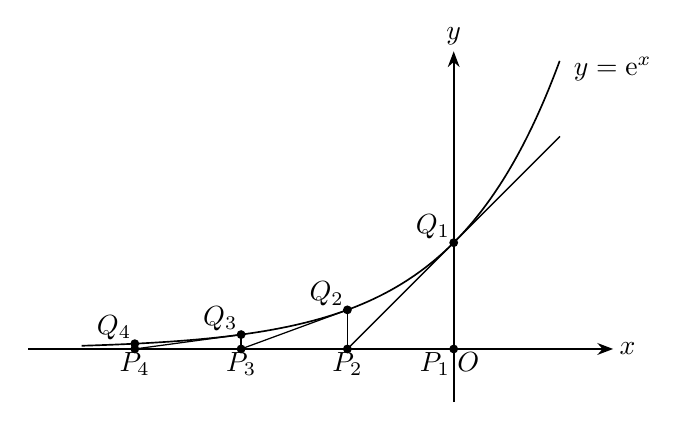
\begin{tikzpicture}[x=1cm,y=1cm,line width=.6pt,>=Stealth,font=\normalsize]
\coordinate (O) at (0,0);
\coordinate (P1) at (0,0);
\coordinate (P2) at (-1.35,0);
\coordinate (P3) at (-2.7,0);
\coordinate (P4) at (-4.05,0);
\coordinate (Q1) at (0,1.35);
\coordinate (Q2) at (-1.35,0.4966372456);
\coordinate (Q3) at (-2.7,0.1827026324);
\coordinate (Q4) at (-4.05,0.0672125423);
\coordinate (T1) at (1.35,2.7);
\draw[->] (-5.4,0)--(2.025,0);
\draw[->] (0,-0.675)--(0,3.78);
\node[right,inner sep=0pt,xshift=2pt] at (2.025,0) {$x$};
\node[above,inner sep=0pt,yshift=2pt] at (0,3.78) {$y$};
\draw[domain=-3.5:1.0,samples=241] plot ({1.35*\x},{1.35*exp(\x)});
\draw[line width=.45pt] (P2)--(T1);
\draw[line width=.45pt] (P3)--(Q2);
\draw[line width=.45pt] (P4)--(Q3);
\draw[line width=.45pt] (P2)--(Q2);
\draw[line width=.45pt] (P3)--(Q3);
\draw[line width=.45pt] (P4)--(Q4);
\fill (P1) circle (1.6pt);
\fill (P2) circle (1.6pt);
\fill (P3) circle (1.6pt);
\fill (P4) circle (1.6pt);
\fill (Q1) circle (1.6pt);
\fill (Q2) circle (1.6pt);
\fill (Q3) circle (1.6pt);
\fill (Q4) circle (1.6pt);
\node[below right,inner sep=1pt] at (O) {$O$};
\node[below left,inner sep=1pt] at (P1) {$P_1$};
\node[below,inner sep=1pt] at (P2) {$P_2$};
\node[below,inner sep=1pt] at (P3) {$P_3$};
\node[below,inner sep=1pt] at (P4) {$P_4$};
\node[above left,inner sep=1pt] at (Q1) {$Q_1$};
\node[above left,inner sep=1pt] at (Q2) {$Q_2$};
\node[above left,inner sep=1pt] at (Q3) {$Q_3$};
\node[above left,inner sep=1pt] at (Q4) {$Q_4$};
\node[anchor=west,inner sep=1pt] at (1.48,3.55) {$y=\mathrm{e}^{x}$};
\end{tikzpicture}
